\subsection{Schritt 3: Non-Maximum Suppression}
\label{sec:impl_non-maximum-suppression}

Die Non-Maximum Suppression wird im CUDA-Kernel
\texttt{non\_maximum\_suppression()} umgesetzt. Jeder Thread ist dabei für
genau einen Pixel zuständig, die Thread-Position ergibt sich wie in
Schritt~1 und~2 aus \texttt{blockIdx} und \texttt{threadIdx}. Als Input
erhält der Kernel den Gradientenbetrag (\texttt{magnitude\_buffer}) sowie
die Gradientenrichtung in Radiant (\texttt{direction\_buffer}) aus
Schritt~2.

Zunächst wird die Gradientenrichtung von Radiant in Grad umgerechnet und
auf den Bereich $[0^\circ, 180^\circ)$ gefaltet, da eine Kante keine
Orientierung besitzt, eine Kante bei $170^\circ$ und eine bei $-10^\circ$
beschreiben dieselbe Achse. Anschließend wird die Richtung auf eine von
vier Klassen quantisiert, die den vier möglichen Achsen im diskreten
Pixelraster entsprechen (siehe Abbildung~\ref{fig:nms_directions}).

Je nach Richtungsklasse werden die Offsets $(dx, dy)$ zum Nachbarpixel
bestimmt (Listing~\ref{lst:nms_kernel}, Zeile~18--22). Der Pixel überlebt
die Suppression genau dann, wenn seine Magnitude größer oder gleich beiden
Nachbarn entlang dieser Achse ist (Zeile~24--26), andernfalls wird er auf
null gesetzt:

\begin{lstlisting}[style=cuda, basicstyle=\ttfamily\scriptsize,
    caption={non\_maximum\_suppression Kernel},
    label={lst:nms_kernel}, numbers=left]
__global__ void non_maximum_suppression(
    const uint8_t* magnitude_buffer,
    const float* direction_buffer,
    const int32_t width,
    const int32_t height,
    uint8_t* out_nms_buffer)
{
    const auto x = static_cast<int32_t>(blockIdx.x * blockDim.x + threadIdx.x);
    const auto y = static_cast<int32_t>(blockIdx.y * blockDim.y + threadIdx.y);
    if (x >= width || y >= height)
        return;

    const uint8_t magnitude = magnitude_buffer[y * width + x];
    const float direction = direction_buffer[y * width + x];

    float deg = direction * (180.0f / CUDART_PI_F);
    deg = fmodf(deg + 180.0f, 180.0f);

    int32_t dx, dy;
    if (deg < 22.5f)       { dx = 1; dy =  0; }
    else if (deg < 67.5f)  { dx = 1; dy = -1; }
    else if (deg < 112.5f) { dx = 0; dy =  1; }
    else if (deg < 157.5f) { dx = 1; dy =  1; }
    else                   { dx = 1; dy =  0; }

    const uint8_t neighbor_a =
        sample_clamped(magnitude_buffer, width, height, x + dx, y + dy);
    const uint8_t neighbor_b =
        sample_clamped(magnitude_buffer, width, height, x - dx, y - dy);

    out_nms_buffer[y * width + x] =
        (magnitude >= neighbor_a && magnitude >= neighbor_b) ? magnitude : 0;
}
\end{lstlisting}

\begin{figure}[H]
    \centering
    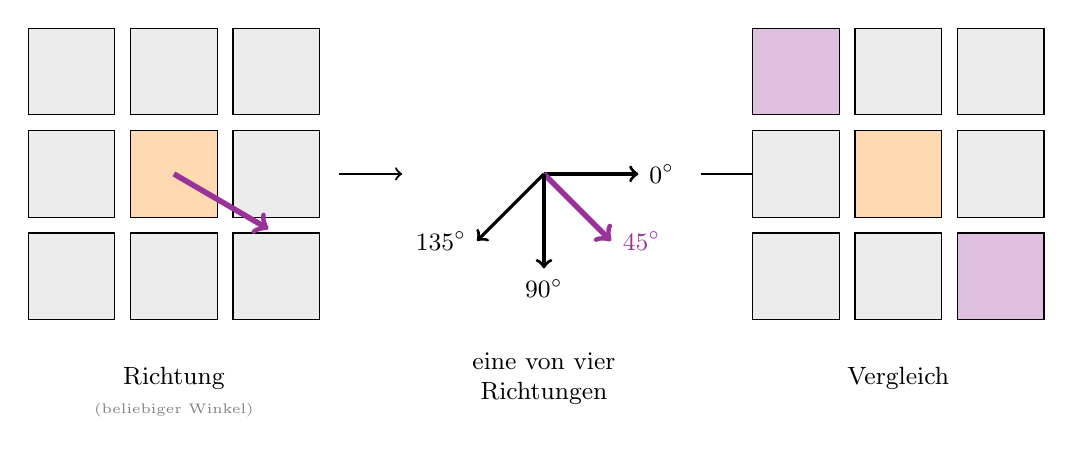
\begin{tikzpicture}[
        pixel/.style={rectangle, draw, minimum size=1.1cm, align=center,
        font=\small, inner sep=2pt, fill=gray!15},
        center/.style={rectangle, draw, minimum size=1.1cm, align=center,
        font=\small\bfseries, inner sep=2pt, fill=orange!30},
        n_violet/.style={rectangle, draw, minimum size=1.1cm, align=center,
        font=\small, inner sep=2pt, fill=violet!25},
    ]

        %% Panel 1: Richtung
        \foreach \col in {0,1,2} {
            \foreach \row in {0,1,2} {
                \node[pixel] at (\col*1.3, -\row*1.3) {};
            }
        }
        \node[center] at (1.3,-1.3) {};
        \draw[->, line width=2pt, violet!80] (1.3,-1.3) -- (2.5,-2.0);
        \node[font=\small] at (1.3,-3.9) {Richtung};
        \node[font=\tiny, text=gray] at (1.3,-4.3) {(beliebiger Winkel)};

        %% Pfeil
        \draw[->, thick] (3.4,-1.3) -- (4.2,-1.3);

        %% Panel 2: 4 Richtungen
        \coordinate (O) at (6.0,-1.3);
        \draw[->, very thick, black]         (O) -- ++(1.2, 0)       node[right, font=\small] {$0^\circ$};
        \draw[->, line width=2pt, violet!80] (O) -- ++(0.85,-0.85)   node[right, font=\small] {$45^\circ$};
        \draw[->, very thick, black]         (O) -- ++(0,-1.2)       node[below, font=\small] {$90^\circ$};
        \draw[->, very thick, black]         (O) -- ++(-0.85,-0.85)  node[left,  font=\small] {$135^\circ$};
        \node[font=\small, align=center] at (6.0,-3.9) {eine von vier\\Richtungen};

        %% Pfeil
        \draw[->, thick] (8.0,-1.3) -- (8.8,-1.3);

        %% Panel 3: Vergleich
        \foreach \col in {0,1,2} {
            \foreach \row in {0,1,2} {
                \node[pixel] at (9.2+\col*1.3, -\row*1.3) {};
            }
        }
        \node[center]   at (9.2+1.3, -1.3) {};
        \node[n_violet] at (9.2+2.6, -2.6) {};   % SE
        \node[n_violet] at (9.2+0,    0)   {};   % NW
        \node[font=\small] at (9.2+1.3,-3.9) {Vergleich};

    \end{tikzpicture}
    \caption{Non-Maximum Suppression: Die Gradientenrichtung wird auf eine von
    vier Achsen quantisiert ($0^\circ$, $45^\circ$, $90^\circ$, $135^\circ$).
    Anschließend wird der Pixel mit den beiden farbig markierten Nachbarn entlang
    der gewählten Achse verglichen.}
    \label{fig:nms_directions}
\end{figure}

Das Ergebnis der Non-Maximum Suppression ist in
Abbildung~\ref{fig:nms_result} dargestellt. Im Vergleich zur
Gradientenmagnitude aus Schritt~2 sind die Kanten auf eine Breite von
einem Pixel reduziert.

\begin{figure}[H]
    \centering
    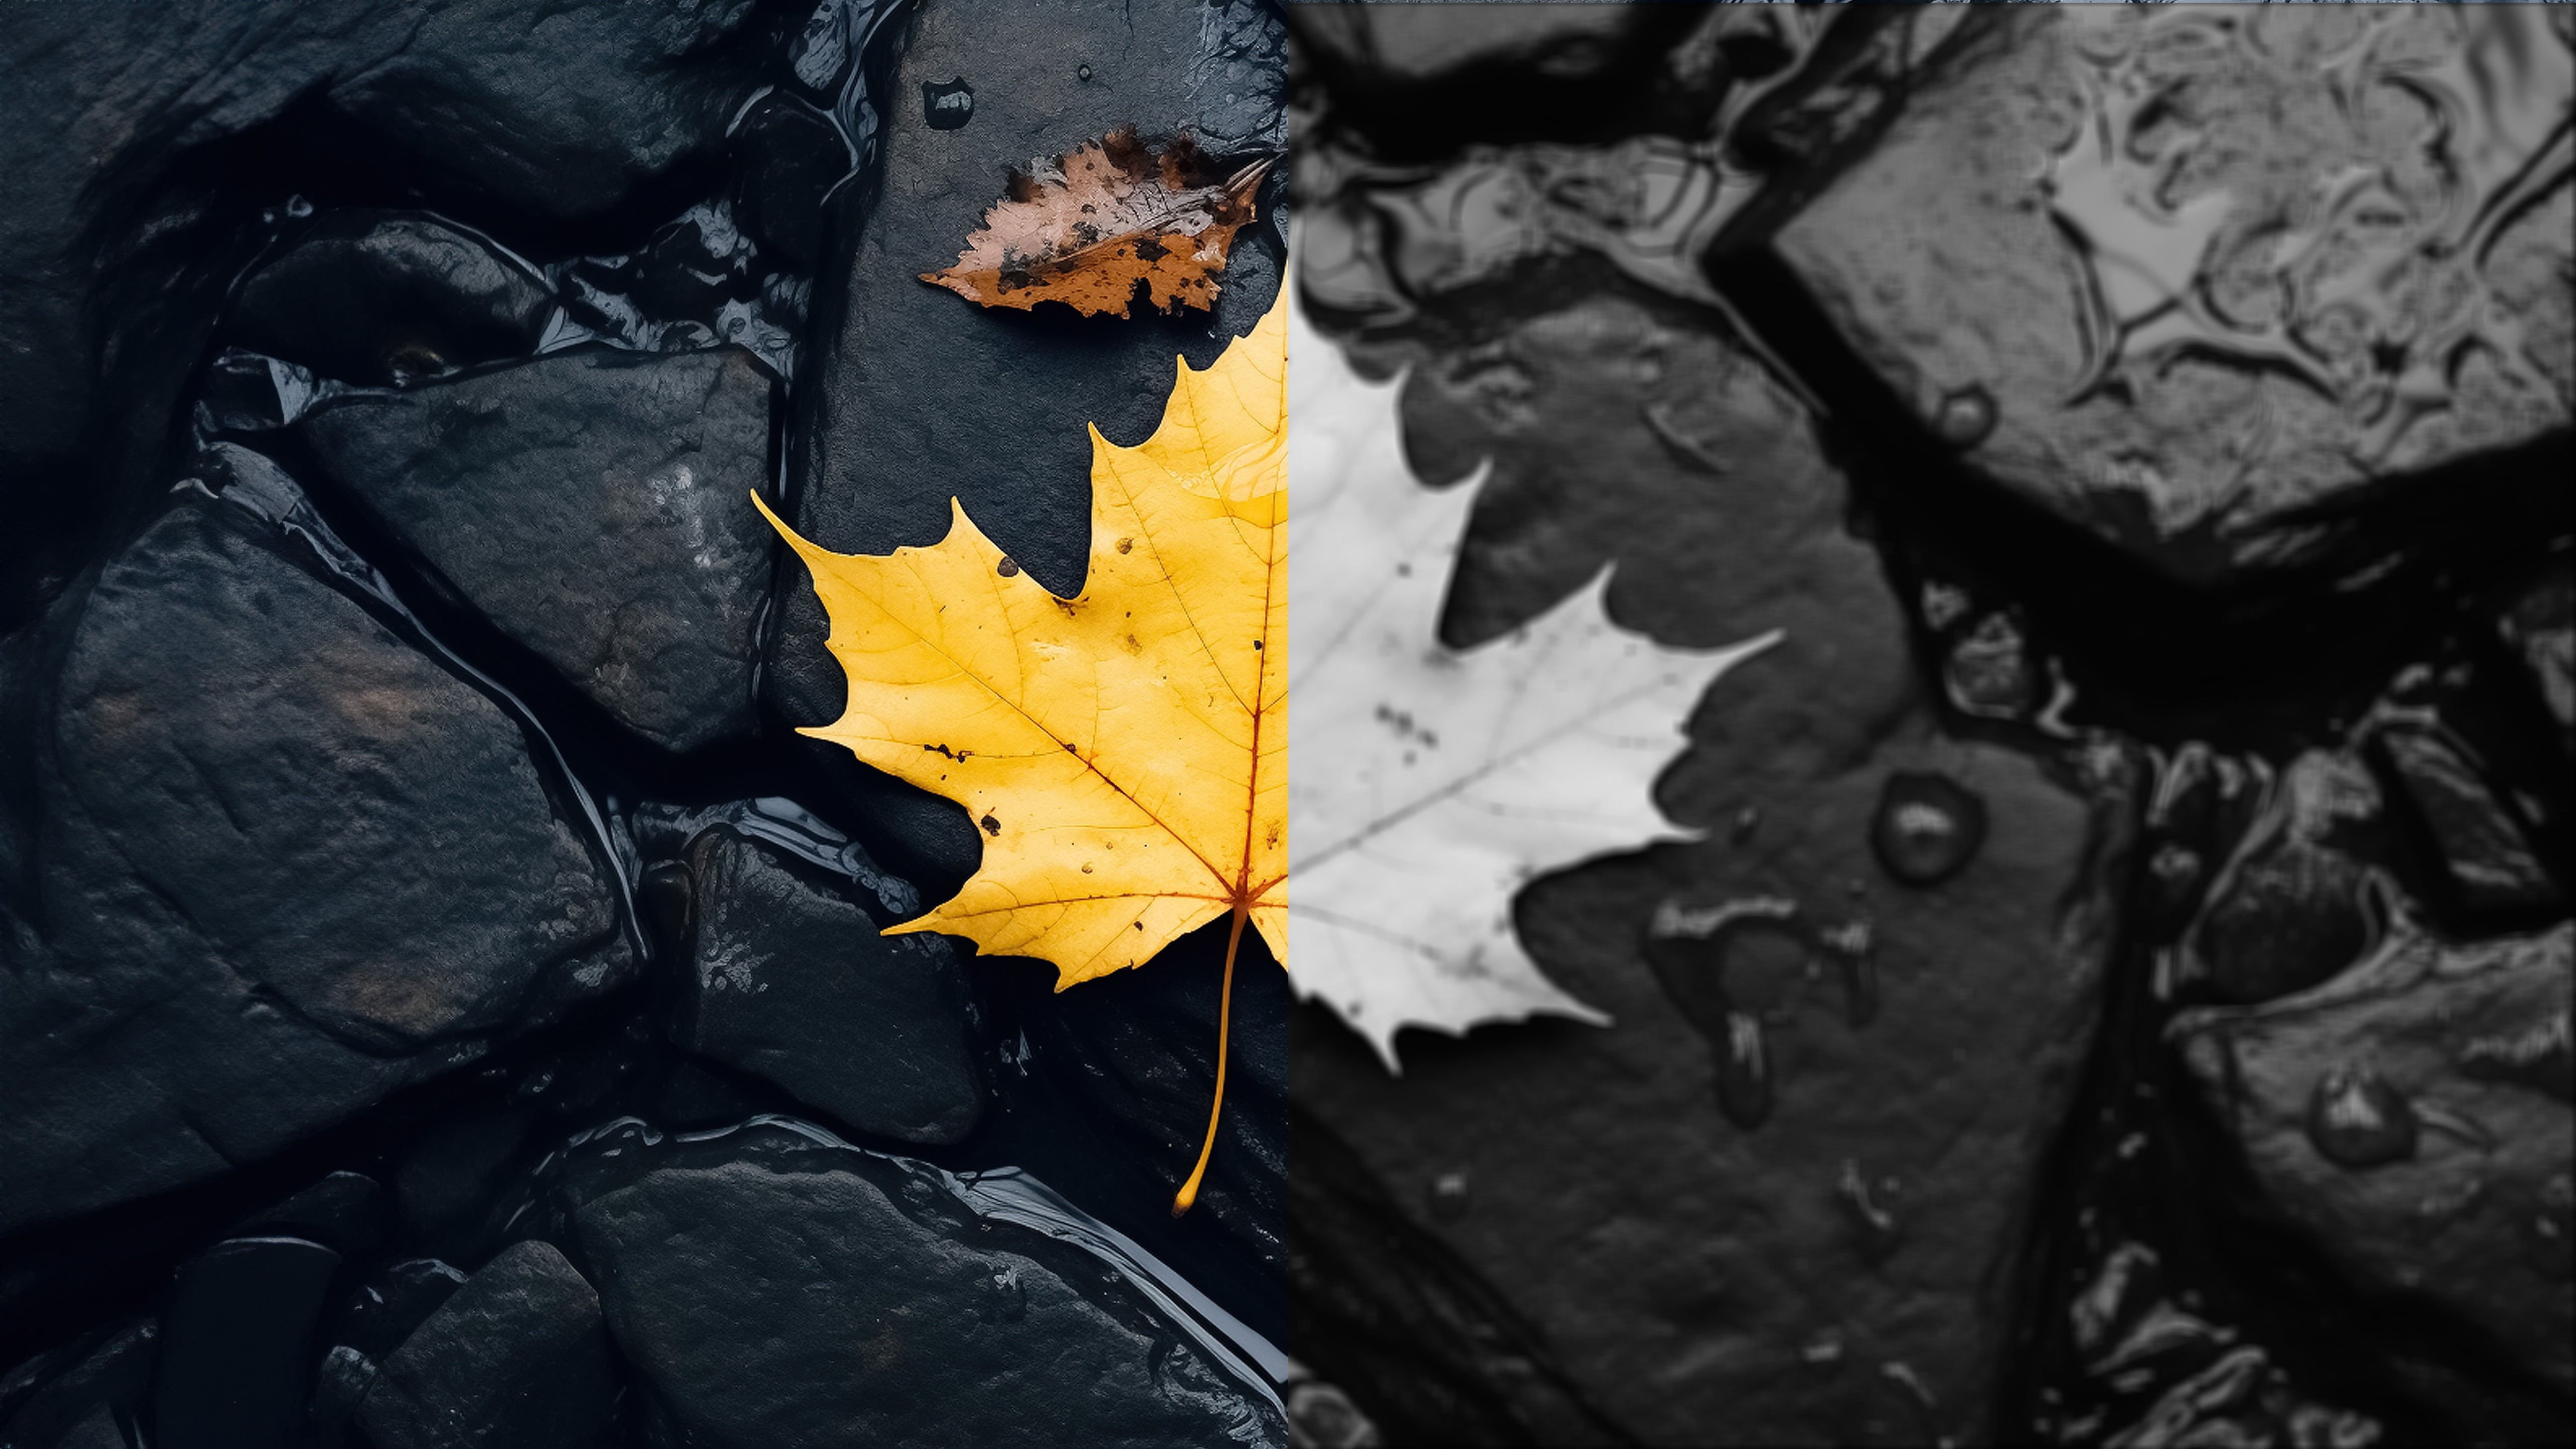
\includegraphics[width=0.7\textwidth]{98_assets/maple-leaf-black-5120x2880-cmp-original-gaussian.jpg}
    \caption{Vergleich Gradientenmagnitude (links) vs.\ Non-Maximum
    Suppression (rechts), die breite Gradientenantwort wird auf
    eine Breite von einem Pixel reduziert. (Placeholder -- wird ersetzt)}
    \label{fig:nms_result}
\end{figure}